\documentclass [11pt, a4paper, oneside] {article}
\usepackage {amsmath}
\usepackage {geometry}
\geometry{left=2.5cm,right=2.5cm}
\usepackage {amssymb}
\usepackage {graphicx}
\usepackage{multirow}
\usepackage[procnames]{listings}
\usepackage{color}
\author {Yue Wang, A53102167}
\title {CSE250A Homework1 Answer}
\begin {document}
\maketitle
\section *{1.1 Conditioning on background evidence}
\subsection *{(a)}
\begin {align*}
\textrm {Right} &= P(X|Y, E)P(Y|E)\\
&= \frac{P(X|Y, E)P(Y|E)P(E)}{P(E)}\\
&= \frac{P(X|Y, E)P(Y, E)}{P(E)} \qquad \qquad&\textrm{(Product Rule)} \\
&= \frac{P(X, Y, E)}{P(E)} &\textrm{(Product Rule)} \\
&= P(X, Y|E) &\textrm{(Product Rule)} \\
&=\textrm {Left} &
\end {align*}
\subsection *{(b)}
\begin {align*}
\textrm {Right} &= \frac{P(Y|X, E)P(X|E)}{P(Y|E)} & \\
& = \frac{P(Y|X, E)P(X|E)P(E)}{P(Y|E)P(E)} & \\
& = \frac{P(Y|X, E)P(X, E)}{P(Y, E)} \qquad \qquad &\textrm{(Product Rule)} \\
& = \frac{P(X, Y, E)}{P(Y, E)} &\textrm{(Product Rule)} \\
& = P(X|Y, E) & \\
& = \textrm {Left} \\
\end {align*}
\section * {1.2 Conditional independence}
\begin {align}
P(X, Y|E) &= P(X|E)P(Y|E)\\
P(X| Y, E) &= P(X|E) \\
P(Y| X, E) &= P(Y|E) 
\end {align}
The thing we need to do is to show (1)$\to$(2)(3), (2)$\to$(1)(3), (3)$\to$(1)(2)\\
\subsubsection *{With (1):}
\begin {align*}
P(X, Y|E) &= P(X|E)P(Y|E) \\
P(X, Y|E)P(E) &= P(X|E)P(Y|E)P(E) \\
P(X, Y, E) &= P(X|E)P(Y, E) \\
P(X|Y, E) &= P(X|E) \\
\end {align*}
(1)$\to$(2)\\
\begin {align*}
P(X, Y|E) &= P(X|E)P(Y|E) \\
P(X, Y|E)P(E) &= P(X|E)P(E)P(Y|E) \\
P(X, Y, E) &= P(X, E)P(Y|E) \\
P(Y|X, E) &= P(Y|E) \\
\end {align*}
(1)$\to$(3)\\
\subsubsection *{With (2):}
\begin {align*}
P(X|Y, E) &= P(X|E)\\
P(X|Y, E)*P(Y|E) &= P(X|E)P(Y|E) \\
P(X, Y|E) &= P(X|E)P(Y|E) \\
\end {align*}
(2)$\to$(1)\\
\begin {align*}
P(X|Y, E) &= P(X|E) \\
\frac{P(Y|X, E)P(X|E)}{P(Y|E)} &= P(X|E) \\
P(Y|X, E) &= P(Y|E)\\
\end {align*}
(2)$\to$(3)\\
\subsubsection*{With (3):}
\begin {align*}
P(Y|X, E) &= P(Y|E) \\
P(Y|X, E)P(X|E) &= P(Y|E)P(X|E) \\
P(X, Y|E) &= P(X|E)P(Y|E) \\
\end {align*}
(3)$\to$(1)\\
\begin {align*}
P(Y|X, E) &= P(Y|E) \\
\frac{P(X|Y, E)P(Y|E)}{P(X|E)} &= P(Y|E) \\
P(X|Y, E) &= P(X|E) \\
\end {align*}
(3)$\to$(2)\\

One equation can be derived from others, so the three equations are equivalent.
\section *{1.3 Creative writing}
\subsection *{(a)}
Y = Bell completed the first assignment\\
Z = Bell completed the second assignment\\
X = Bell passed the course\\

$P(X = 1) < P(X=1|Y=1) < P(X = 1|Y=1, Z=1)$\\

Using our common sense, we have more confidence in a student passing a course when we know he completed two assignments than that when we know he completed one assignment, which is more than that when we don't know whether he did assignment or not.\\
\subsection *{(b)}
X = Bell completed the first assignment\\
Z = Bell completed the second assignment\\
Y = Bell passed the course\\

$P(X=1|Y=1) > P(X=1)$\\

$P(X=1|Y=1, Z=1) < P(X=1|Y=1)$\\

Because we have more confidence in that Bell completed the first assignment when we know he passed the course. And Bell completing the second assignment "explains away" the Bell passing the course, thus decreasing our belief in Bell completing the first assignment.\\
\subsection *{(c)}
X = Mary calls \\
Y = Bell calls \\ 
Z = Alarm goes off \\

$P(X=1, Y=1) \neq P(X=1)P(Y=1)$\\

$P(X=1, Y=1|Z=1) = P(X=1|Z=1)P(Y=1|Z=1)$\\

These events are from the lecture. Because Mary calling and Bell calling both depend on whether alarm going off, which gives us the first inequation. But when we know the alarm goes off, Mary calling and Bell calling are independent. \\
\section *{1.4 Bayes Rule}
$\textrm{From the question, we know two events, which are represented in the below way:}\\
\textrm{X = Cyclists using performance-enhancing drugs}\\
\textrm{Y = The drug test is positive}\\
P(X=1) = 0.01\qquad P(Y=1|X=0) = 0.05\qquad P(Y=0|X=1) = 0.1\\
\textrm{From the above, we can derive:}\\
P(X=0) = 0.99 \qquad P(Y=0|X=0) = 0.95\qquad P(Y=1|X=1) = 0.9\\
P(Y=0) = P(Y=0, X=0) + P(Y=0, X=1) = P(Y=0|X=0)*P(X=0) + P(Y=0|X=1)*P(X=1) = 0.9415\\
P(Y=1) = 0.0585$\\
\subsection *{(a)}
$\textrm{This question is to compute }P(X=0|Y=0)$\\
$P(X=0|Y=0) = \frac{P(Y=0|X=0)P(X=0)}{P(Y=0)} = \frac{0.95*0.99}{0.9415} \approx 0.9989$\\
\subsection *{(b)}
$\textrm{This question is to compute }P(X=1|Y=1)$\\
$P(X=1|Y=1) = \frac{P(Y=1|X=1)P(X=1)}{P(Y=1)} = \frac{0.9*0.01}{0.0585} \approx 0.1538$\\
\section* {1.5 Entropy}
\subsection *{(a)}
$\textrm{Let } f(x) = H(X) + \lambda(\sum_{i}p_i -1)$\\
$\textrm{If we want to get  maximum of H(X) under the constraint that }\sum_{i}p_i=1$,\\
$\textrm{we just need to get the maximum of f(x) }$\\
$\frac{\partial{f}}{\partial{p_i}} = -1-\log{p_i}+\lambda \textrm{, for all i}$\\
$\frac{\partial{f}}{\partial{\lambda}}= \sum_{i}p_i - 1 $\\
$\textrm{Let } \frac{\partial{f}}{\partial{p_i}} = 0, \frac{\partial{f}}{\partial{\lambda}} = 0$\\
$\textrm{We got } p_i = e^{\lambda-1} \textrm{ for all i, }and \sum_{i}p_i=1$\\
$\textrm{Finally we got } p_i = \frac{1}{n} \textrm{ and } \lambda = \log{\frac{1}{n}} + 1\textrm{, for all i}\\ \textrm{And after testing, we find}(\frac{1}{n},\frac{1}{n}, \cdots, \frac{1}{n})\textrm{ is the maximum point.}$\\
\subsection *{(b)}
If we know $X_1, X_2, ..., X_n$ are independent, then\\
$H(X_1, X_2, ..., X_n) = -\sum_{x_1}\sum_{x_2}\cdots\sum_{x_n}P(x_1)P(x_2)\cdots P(x_n)\log{P(x_1)P(x_2)\cdots P(x_n)}$\\
$H(X_1, X_2, ..., X_n) = -\sum_{x_1}\sum_{x_2}\cdots\sum_{x_n}P(x_1)P(x_2)\cdots P(x_n)(\log{P(x_1)}+\log{P(x_2)}+\cdots+\log{P(x_n))}$\\
$H(X_1, X_2, ..., X_n) = -\sum_{x_1}\sum_{x_2}\cdots\sum_{x_n}P(x_1)P(x_2)\cdots P(x_n)\log{P(x_1)} \\
-\sum_{x_1}\sum_{x_2}\cdots\sum_{x_n}P(x_1)P(x_2)\cdots P(x_n)\log{P(x_2)}\\
-\cdots-\sum_{x_1}\sum_{x_2}\cdots\sum_{x_n}P(x_1)P(x_2)\cdots P(x_n)\log{P(x_n)}$\\
Because the sum calculation is commutative in this case, then\\
$H(X_1, X_2, ..., X_n) = -\sum_{x_2}\cdots\sum_{x_n}P(x_2)\cdots P(x_n)\sum_{x_1}P(x_1)\log{P(x_1)} \\
-\sum_{x_1}\cdots\sum_{x_n}P(x_1)\cdots P(x_n)\sum_{x_2}P(x_2)\log{P(x_2)}\\
-\cdots-\sum_{x_1}\sum_{x_2}\cdots\sum_{x_n-1}P(x_1)P(x_2)\cdots P(x_n-1)\sum_{x_n}P(x_n)\log{P(x_n)}$\\
$H(X_1, X_2, ..., X_n) = \sum_{x_2}\cdots\sum_{x_n}P(x_2)\cdots P(x_n)H(X_1) \\
+\sum_{x_1}\cdots\sum_{x_n}P(x_1)\cdots P(x_n)H(X_2)\\
+\cdots+\sum_{x_1}\sum_{x_2}\cdots\sum_{x_n-1}P(x_1)P(x_2)\cdots P(x_n-1)H(X_n)$\\
$H(X_1, X_2, ..., X_n) = \sum_{x_2}\cdots\sum_{x_n-1}P(x_2)\cdots P(x_n-1)\sum_{x_n} P(x_n)H(X_1) \\
+\sum_{x_1}\sum_{x_3}\cdots\sum_{x_n-1}P(x_1)P(x_3)\cdots P(x_n-1)\sum_{x_n}P(x_n)H(X_2)\\
+\cdots+\sum_{x_1}\sum_{x_2}\cdots\sum_{x_n-2}P(x_1)P(x_2)\cdots P(x_n-2)\sum_{x_n-1} P(x_n-1)H(X_n)$\\
$H(X_1, X_2, ..., X_n) = \sum_{x_2}\cdots\sum_{x_n-1}P(x_2)\cdots P(x_n-1)H(X_1) \\
+\sum_{x_1}\sum_{x_3}\cdots\sum_{x_n-1}P(x_1)P(x_3)\cdots P(x_n-1)H(X_2)\\
+\cdots+\sum_{x_1}\sum_{x_2}\cdots\sum_{x_n-2}P(x_1)P(x_2)\cdots P(x_n-2)H(X_n)$\\
$\cdots$ \\
$\cdots$ \\
$H(X_1, X_2, ..., X_n) = H(X_1) + H(X_2) + \cdots + H(X_n) = \sum_{i=1}^{n}H(X_i)$\\
\section *{1.6 Kullback-Leibler distance}
\subsection *{(a)}
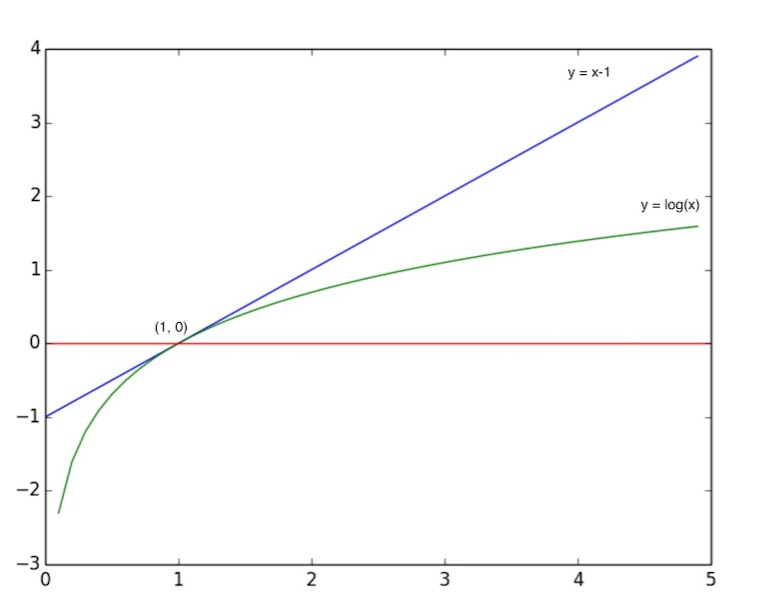
\includegraphics[height=5cm]{figure.jpg}\\
$\textrm{Let }f(x) = \log(x) - (x-1)\qquad (x > 0)$\\
$\frac{df(x)}{dx} = \frac{1}{x} - 1\qquad (x>0)$\\
$\textrm{When }0 < x < 1, \frac{df(x)}{dx} > 0. \textrm{When }x = 1, \frac{df(x)}{dx} = 0. \textrm{When }x > 1, \frac{df(x)}{dx} = <0. $\\
So when $0 < x < 1, f(x)$ increases, when $x > 1, f(x)$ decreases and when $x=1, f(x)$ is the maximum value. $f(0) = 0$ \\
So $\log(x) <= x - 1$ with equality if and only if $x = 1$. \\
\subsection *{(b)}
We know $\log(x) <= x -1$ with equality if and only if $x = 1$\\
Let $ x = \frac{q_i}{p_i},\textrm{for all i}$, we have:\\
$\log(\frac{q_i}{p_i}) <= \frac{q_i}{p_i} - 1,  \textrm{for all i}$\\
$p_i\log(\frac{q_i}{p_i}) <= q_i - p_i,\textrm{for all i}\qquad\textrm{(We know }p_i >= 0)$\\
$p_i - q_i <= p_i\log(\frac{p_i}{q_i}), \textrm{for all i}$\\
$\sum{(p_i - q_i)} <= \sum_i{p_i\log(\frac{p_i}{q_i})}$\\
$\sum{p_i} -\sum{q_i} <= \sum_i{p_i\log(\frac{p_i}{q_i})}$\\
$1 - 1 <= \sum_i{p_i\log(\frac{p_i}{q_i})}$\\
$KL(p, q) >= 0, \textrm{and when the two distributions are equal, }\log(1) = 0, \\ \textrm{so every term in the KL is 0 when two distributions are equal}$\\
$KL(p, q) >= 0, \textrm{with equality if and only if the two distributions are equal}$\\
\subsection *{(c)}
We know $\log(x) <= x -1$ with equality if and only if $x = 1$\\
Let $ x = \frac{\sqrt{q_i}}{\sqrt{p_i}},\textrm{for all i}$, we have:\\
$\log(\frac{\sqrt{q_i}}{\sqrt{p_i}}) <= \frac{\sqrt{q_i}}{\sqrt{p_i}} - 1,  \textrm{for all i}$\\
$p_i\log(\frac{\sqrt{q_i}}{\sqrt{p_i}}) <= p_i(\frac{\sqrt{q_i}}{\sqrt{p_i}} - 1),  \textrm{for all i}$\\
$2p_i\log(\frac{\sqrt{q_i}}{\sqrt{p_i}}) <= 2p_i(\frac{\sqrt{q_i}}{\sqrt{p_i}} - 1),  \textrm{for all i}$\\
$p_i\log(\frac{q_i}{p_i}) <= 2\sqrt{p_i q_i} - 2p_i,  \textrm{for all i}$\\
$\sum_ip_i\log(\frac{p_i}{q_i}) >=  \sum_i(2p_i - 2\sqrt{p_i q_i})$\\
$\sum_ip_i\log(\frac{p_i}{q_i}) >=  \sum_i(p_i - 2\sqrt{p_i q_i} + p_i)\qquad\textrm{Because } \sum_i{p_i} = \sum_{q_i} = 1$\\
$\sum_ip_i\log(\frac{p_i}{q_i}) >=  \sum_i(\sqrt{p_i} - \sqrt{p_i})^2$\\
$KL(p, q) >=  \sum_i(\sqrt{p_i} - \sqrt{p_i})^2$\\
\subsection *{(d)}
Let p = Tomorrow will rain.\\
Let q = Earthquake occurs.\\
$
P(p = 1) = 0.3\\
P(p = 0) = 0.7\\
P(q = 1) = 0.1\\
P(q = 0) = 0.9\\
KL(p, q) \approx 0.1537 \\
KL(q, p) \approx 0.1163 \\
KL(p, q) \neq KL(q, p) \\
$
\section *{1.7 Hangman}
\subsection *{(a)}
The eight most frequent 5-leter words (with their probabilities) are:\\
('THREE', 0.03562714868653127), ('SEVEN', 0.023332724928853858), \\('EIGHT', 0.021626496097709325), ('WOULD', 0.02085818430793947), \\('ABOUT', 0.020541544349751077), ('THEIR', 0.018974130893766185), \\('WHICH', 0.018545160072784138), ('AFTER', 0.01436452108630337) \\
The fourteen(There are 9 words whose frequence are 7 with the same probability) least frequent 5-leter words (with their probabilities) are:\\
('TROUP', 7.827934689453437e-07), ('MAPCO', 7.827934689453437e-07), \\('CAIXA', 7.827934689453437e-07), ('BOSAK', 7.827934689453437e-07), \\('OTTIS', 7.827934689453437e-07), ('NIAID', 9.13259047102901e-07), \\('SERNA', 9.13259047102901e-07), ('CLEFT', 9.13259047102901e-07),\\ ('CCAIR', 9.13259047102901e-07), ('FABRI', 9.13259047102901e-07), \\('FOAMY', 9.13259047102901e-07), ('PAXON', 9.13259047102901e-07), \\('TOCOR', 9.13259047102901e-07),
('YALOM', 9.13259047102901e-07)
\subsection *{(b)}
\begin{table}[!hbp]
\begin{tabular}{|c|c|c|c|c|}
\hline
correctly guessed & incorrectly guessed & best next guess $l$ & $P(L_i = l \textrm{ for some i }\in \textrm\{1, 2, 3, 4, 5\textrm\}|E)$\\
\hline
- - - - - & \{\} & E & 0.5394\\
\hline
- - - - - & \{E, O\} & I & 0.6366\\
\hline
D - -I - & \{\} & A & 0.8207\\
\hline
D - -I - & \{A\} & E & 0.7521\\
\hline
-U - - - & \{A, I, E, O, S\} & Y & 0.6270\\
\hline
\end{tabular}
\end{table}
\subsection *{(c)}
\definecolor{keywords}{RGB}{255,0,90}
\definecolor{comments}{RGB}{0,0,113}
\definecolor{red}{RGB}{160,0,0}
\definecolor{green}{RGB}{0,150,0}
 
\lstset{language=Python, 
        basicstyle=\tiny, 
        keywordstyle=\color{keywords},
        commentstyle=\color{comments},
        stringstyle=\color{red},
        numbersep=10pt,
        showstringspaces=false,
        identifierstyle=\color{green},
        procnamekeys={def,class}}
 
\lstinputlisting{hangman.py}
Program output. 
\subsubsection *{1}
('Q', 0.0042710516321439245), ('Z', 0.004292056590227289), ('J', 0.01563055905674421), ('X', 0.020749506481334088), ('K', 0.05958258581993074), ('V', 0.06369355618767535), ('P', 0.0772493211549799), ('B', 0.08609971458045411), ('M', 0.09001668263347834), ('F', 0.104002201215234), ('Y', 0.10544123654231159), ('W', 0.10968606459324606), ('G', 0.11007759179329682), ('C', 0.1490947580626736), ('U', 0.15630976546594258), ('D', 0.17146229864431772), ('L', 0.20103153914025876), ('N', 0.23201711395267857), ('H', 0.2597325690485791), ('I', 0.3025530678524059), ('O', 0.3146699279582104), ('A', 0.34689936159278384), ('S', 0.3498943294049688), ('R', 0.3831019939445695), ('T', 0.43069322754488293), ('E', 0.539417238964795)
\subsubsection *{2}
('E', 0.0), ('O', 0.0), ('Z', 0.004600009630695304), ('Q', 0.008808839896183281), ('J', 0.01151625558566803), ('V', 0.028985687596476063), ('X', 0.04363029600320741), ('B', 0.0780064677152583), ('K', 0.09037433646944139), ('M', 0.10066457208061445), ('W', 0.10232343229323645), ('P', 0.10274977992779151), ('G', 0.11908030106202787), ('D', 0.1265246121075156), ('U', 0.1443002785867984), ('Y', 0.18198713707022385), ('F', 0.18460744366178544), ('C', 0.20778549736319163), ('L', 0.2463845666484698), ('N', 0.2588422497520642), ('H', 0.27253569173551095), ('R', 0.3098751959278396), ('S', 0.42672258241142885), ('A', 0.4425520909700327), ('T', 0.4857500877854112), ('I', 0.6365554141009607)
\subsubsection *{3}
('C', 0.0), ('D', 0.0), ('G', 0.0), ('F', 0.0), ('I', 0.0), ('H', 0.0), ('Q', 0.0), ('W', 0.0), ('Y', 0.0), ('X', 0.0), ('Z', 0.0), ('U', 0.0018601190476190477), ('K', 0.003162202380952381), ('J', 0.006882440476190476), ('P', 0.006882440476190476), ('T', 0.01525297619047619), ('B', 0.017113095238095236), ('M', 0.017857142857142856), ('O', 0.04538690476190476), ('L', 0.07384672619047619), ('E', 0.1408110119047619), ('R', 0.18098958333333331), ('N', 0.18601190476190474), ('S', 0.7395833333333334), ('V', 0.7436755952380953), ('A', 0.8206845238095238)
\subsubsection *{4}
('A', 0.0), ('C', 0.0), ('D', 0.0), ('G', 0.0), ('F', 0.0), ('I', 0.0), ('H', 0.0), ('K', 0.0), ('Q', 0.0), ('W', 0.0), ('Y', 0.0), ('X', 0.0), ('Z', 0.0), ('U', 0.01037344398340249), ('J', 0.03838174273858921), ('P', 0.03838174273858921), ('T', 0.0850622406639004), ('B', 0.0954356846473029), ('M', 0.0995850622406639), ('O', 0.1991701244813278), ('R', 0.237551867219917), ('N', 0.30186721991701243), ('S', 0.37033195020746884), ('L', 0.37551867219917007), ('V', 0.39626556016597503), ('E', 0.7520746887966804)
\subsubsection *{5}
('A', 0.0), ('E', 0.0), ('I', 0.0), ('O', 0.0), ('Q', 0.0), ('S', 0.0), ('U', 0.0), ('W', 0.0), ('X', 0.0), ('J', 0.001577932324235871), ('V', 0.0028052130208637708), ('Z', 0.018759862077026467), ('G', 0.020104026649523692), ('P', 0.05908479925194317), ('M', 0.06574718017649463), ('R', 0.0993512944889252), ('K', 0.10291625270293957), ('B', 0.15644906785108986), ('T', 0.19320904681199222), ('D', 0.274326456665303), ('F', 0.3075214774121909), ('N', 0.3091578516743614), ('H', 0.3877622581964817), ('L', 0.4471392671380981), ('C', 0.4625094968149143), ('Y', 0.6269651101630527)
\end {document}

